\section{System Architecture}
\label{sys:arch}
The black-box testing system can be divided broadly into two modules:
\begin{enumerate}
	\item Data Gathering\\
		The Data Gathering module (shown in Fig. \ref{fig:crawler}) is primarily responsible for the following activities:
		\begin{itemize}
			\item Interface with the UCSB Crawler (Section \ref{Comp:Crawler}) and receive the URLs.
			\item Parse the HTML for the corresponding URL, and store the relevant form data (Section \ref{Comp:FP}).
			\item Check for the presence of forms that allow the user to send/receive E-Mail, and store references to these forms (Section \ref{Comp:EMFC}).
		\end{itemize} 
	\item Payload Injection\\
		The Payload Injection module (shown in Fig. \ref{fig:fuzzer}) is primarily responsible for the following activities:
		\begin{itemize}
			\item Retrieve the forms that allow users of a website to send/receive E-Mail, and reconstruct these forms (Section \ref{Comp:EMFR}).
			\item Inject these forms with benign data (non-malicious payloads), generate a HTTP request to the corresponding URL (Section \ref{Comp:Fuzzer:nmp}).
			\item Analyze the E-Mails, extracting the header fields, and checking for the presence of the injected payloads (Section \ref{Comp:EMA}).
			\item Inject the forms that sent us E-Mails with malicious payloads, generate a HTTP request to the corresponding URL to check if E-Mail Header Injection vulnerability exists in that form (Section \ref{Comp:Fuzzer:mp}).
		\end{itemize} 
	The functionality of each component is discussed further in the `Components' section (\ref{Comp}). It is to be noted that the Payload Injection pipeline is not linear, but is a cyclic process.
\end{enumerate}

\begin{figure}
     \centering
     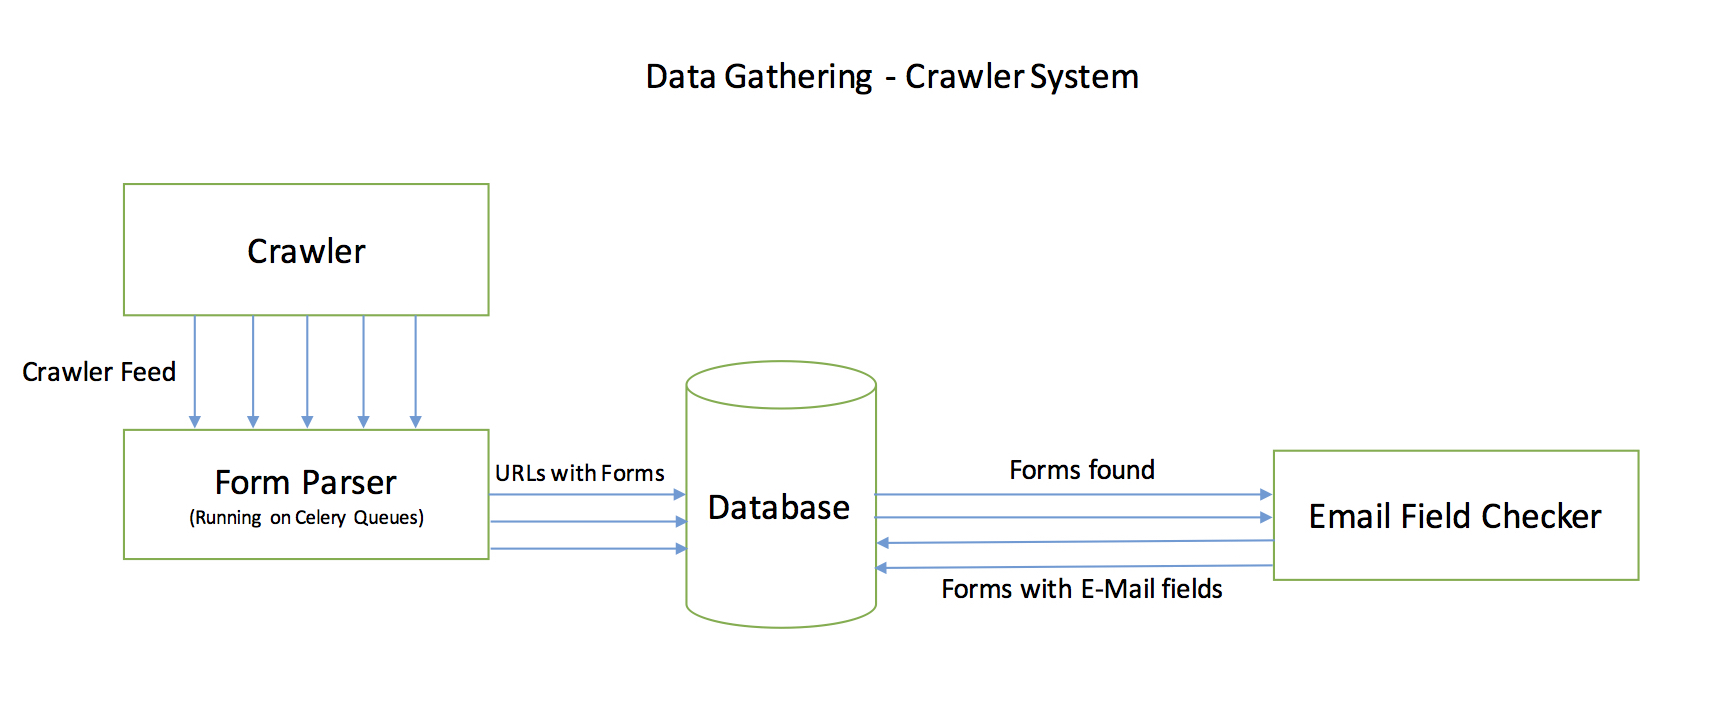
\includegraphics[width=16cm, height=7cm]{System/crawler_design}
     \caption{System Architecture - Crawler}
     \label{fig:crawler}
 \end{figure}
 
 
 \begin{figure}
 	\centering
 	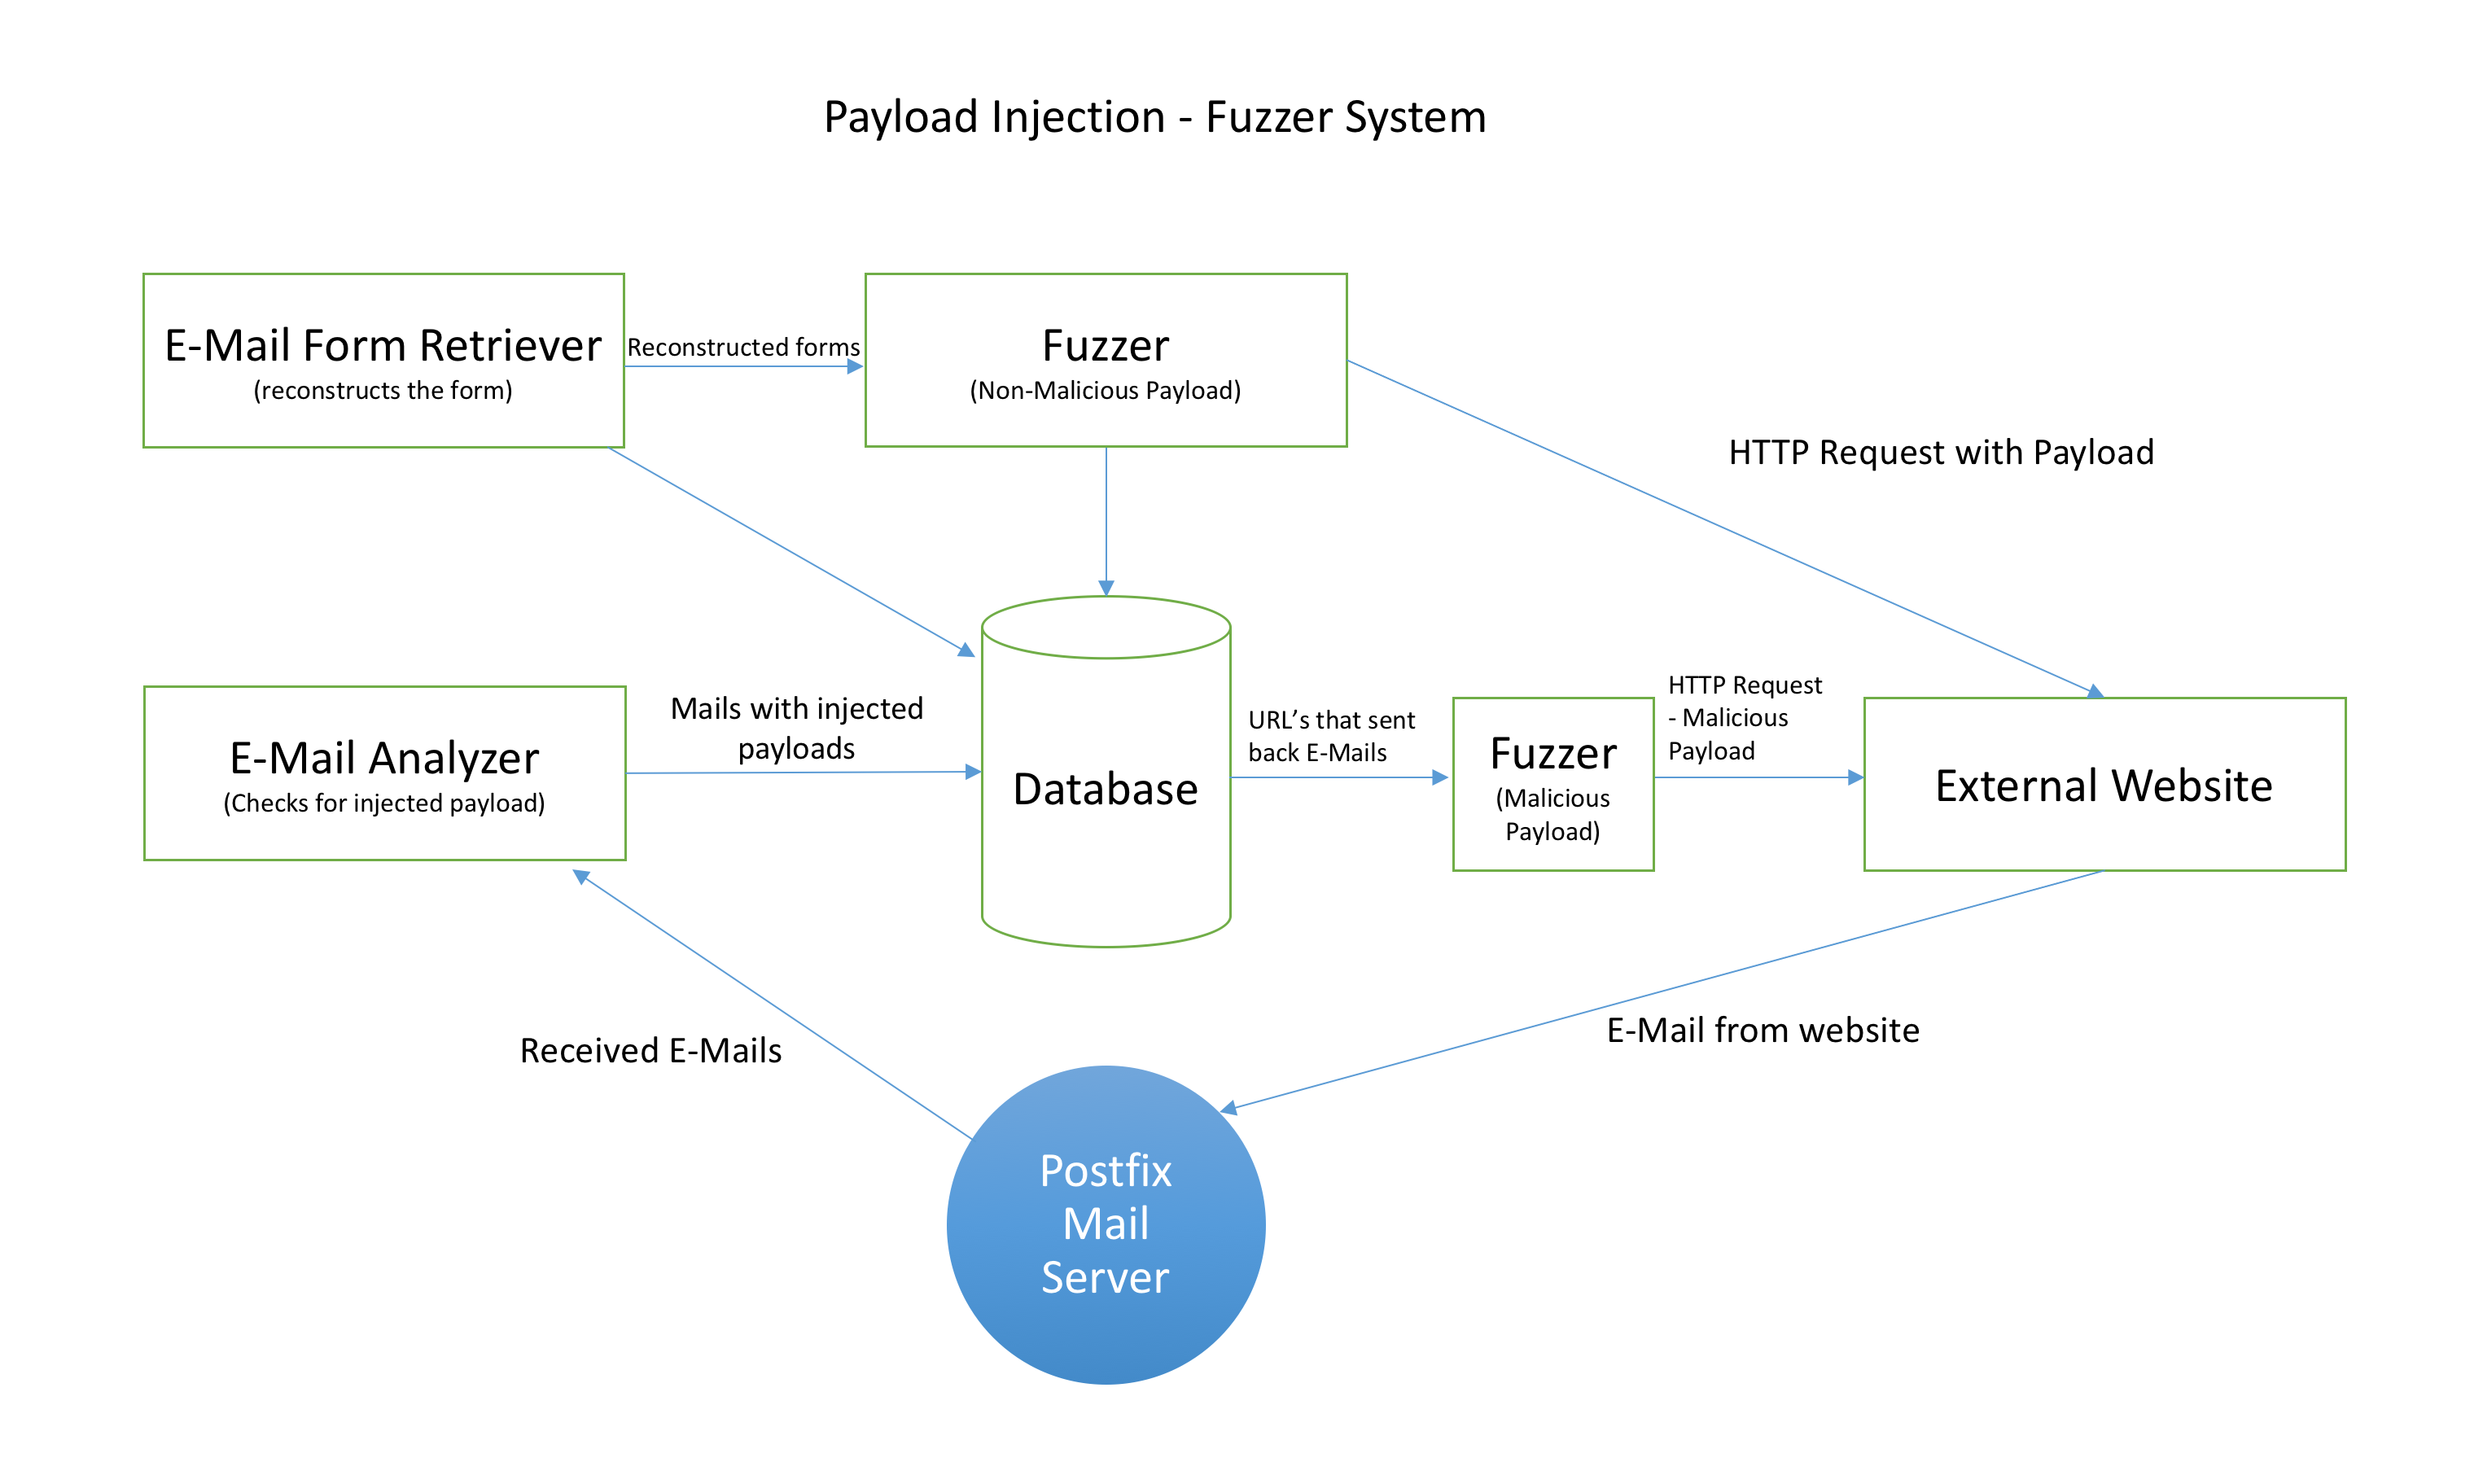
\includegraphics[width=16cm, height=9cm]{System/fuzzer_design}
 	\caption{System Architecture - Fuzzer {\&} E-Mail Analyzer}
 	\label{fig:fuzzer}
 \end{figure}
 